%-----General Settings----%
\documentclass{other/docTemplate}
\svnid{$Id$}

\author{ML: Gonzalo Ducca \formatemail{gonzaloducca@gmail.com} \\ DA: Juan P. Bertone \formatemail{bertonejpb@gmail.com} \\ DE: Juan E. Flórez-Coronel \formatemail{juan.florez@upr.edu} \\ DA: Valentino Caputa \formatemail{caputavalentino@gmail.com} \\ ML: Carlos Madoery \formatemail{ccmadoery@gmail.com}}  
\po{Melina Griffo \formatemail{meligriffo@gmail.com}}
\title{Final Project Report: Life Expectancy} 
\henrymentor{Pía Ruiz \formatemail{mpiaruiz@gmail.com}}

\loadglsentries{other/acronyms}
\makeglossaries

%-----Beginning of Document----%
\begin{document} 
\maketitle

%---Revision Tracker---%
\startTable
\AddRevision{0.0}{10-20-23}{Document Creation}
\AddRevision{1.0}{11-01-23}{Documentation for Sprint 1}
\stopTable

%-----Table of Contents-----%
\tableofcontents
\newpage
\listoftables
\newpage
\listoffigures
\newpage
\printglossary[title=List of Acronyms ,type=\acronymtype]
\clearpage

%-----Acknowledgments-----%
%\section*{Acknowledgments}
%\addcontentsline{toc}{section}{Acknowledgments}%adds acknowledgements section to the table of contents

%Here is a sample for how to susse acronyms. "Defining a \gls{fr} and a \gls{ps} provides a language for system design. This language is an important aspect of \gls{csd}."
%\newpage

%-----Abstract-----%
%\section*{Abstract}
%\addcontentsline{toc}{section}{Abstract}%adds Abstract section to the table of contents
%\newpage

%-----Content-----%
%%%%%%  PROBLEM STATEMENT  %%%%%%                                               
\section{Problem Statement}
We consulted World Bank databases and decided to use as reference key topics that provide indicators influencing the life expectancy of a country's inhabitants. These selected topics are education, health, economy, and the development of science and technology.
We plan to gather indicators from each topic, create the databases we want to work with, and then link these variables to establish relationships. We envision this project as a product that can be offered to a company looking to invest in science and development.
After all the data analysis work is completed, we will create Machine Learning models by specifying certain parameters, such as the percentage of \gls{gdp} invested in education or science. These models will then provide us with an estimated life expectancy for a particular country.

%%%%%%  PROBLEM STATEMENT - Objectives  %%%%%% 
\subsection{Objectives}
To analyze life expectancy in the countries of the Americas based on five factors: 
\begin{itemize}
  \item Education
  \item Health
  \item Economy
  \item Science and Technology
  \item Security
\end{itemize}

%%%%%%  PROBLEM STATEMENT - Possible Clientele  %%%%%% 
\subsection{Possible Clientele}
The potential clientele for this project includes both public and private entities with a vested interest in the subject matter. Public institutions, such as government agencies, can utilize the insights and models generated to inform policy decisions and allocate resources effectively in areas related to education, healthcare, and scientific research. On the other hand, private companies, especially those involved in industries related to science and technology, can benefit from the project's findings when making investment decisions and corporate social responsibility initiatives. This project caters to a broad range of organizations looking to make informed decisions that impact the well-being and development of countries.

%%%%%%   PROBLEM STATEMENT - Scope of the Project %%%%%%  
\subsection{Scope of the Project}
The project scope involves a comprehensive analysis of life expectancy in 30 countries across the World over the past 35 years. This analysis will encompass five key topics within each of the five influencing factors, namely education, health, economy, and science and technology. The goal is to provide a detailed and data-driven insight into the factors that impact life expectancy in these countries over the specified timeframe.



%%%%%%  Data Acquisition %%%%%%  
\clearpage
\section{Data Acquisition}
The data was acquired using the \href{https://datahelpdesk.worldbank.org/knowledgebase/topics/125589}{World Bank API}.

%%%%%%   API %%%%%%  

\subsection{World Bank API}

The World Bank Data has the following topics:

\begin{figure}[htbp!]
  \centering
  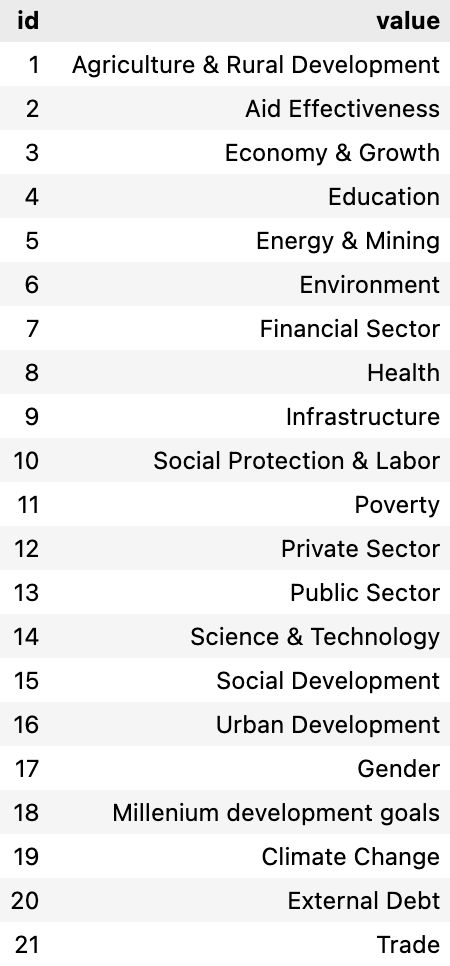
\includegraphics[width=0.4\textwidth]{topics.png}
  \caption{World Bank Data Topics}
  \label{fig:topics}
\end{figure}

And the following economies:

\begin{figure}[htbp!]
  \centering
  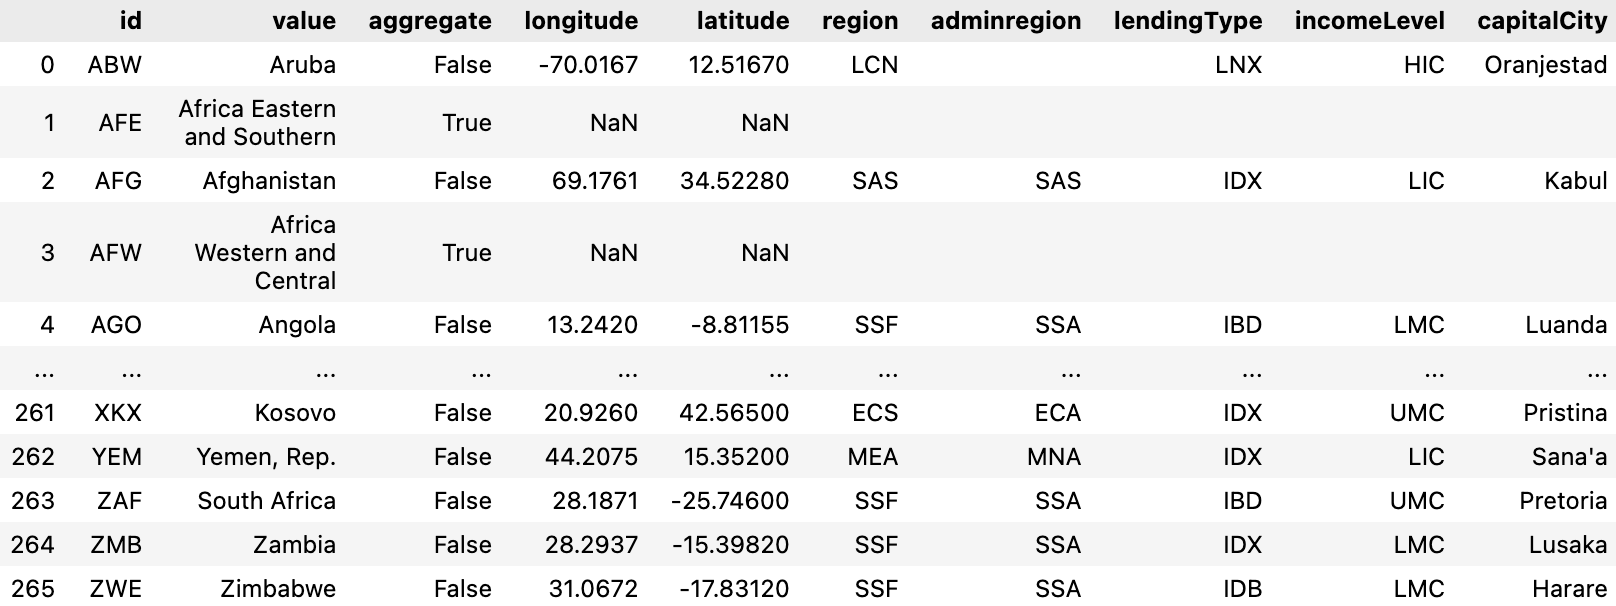
\includegraphics[width=0.9\textwidth]{economies.png}
  \caption{World Bank Data Economies}
  \label{fig:economies}
\end{figure}

Each topic has a few factors:

\begin{figure}[htbp!]
  \centering
  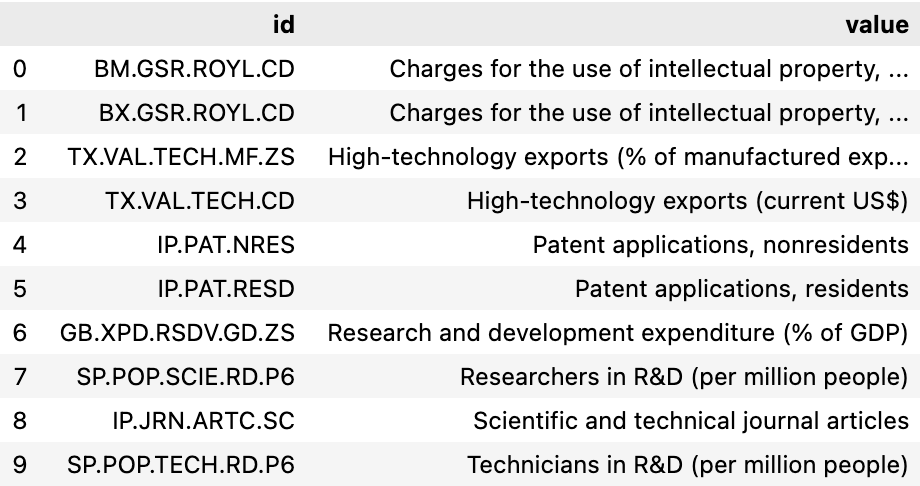
\includegraphics[width=0.7\textwidth]{st_factors.png}
  \caption{World Bank Data Science \& Technology Factors}
  \label{fig:stfactors}
\end{figure}

%%%%%%   Possible Topics %%%%%% 

\subsection{Possible Topics}

Counting missing values:

\begin{figure}[htbp!]
  \centering
  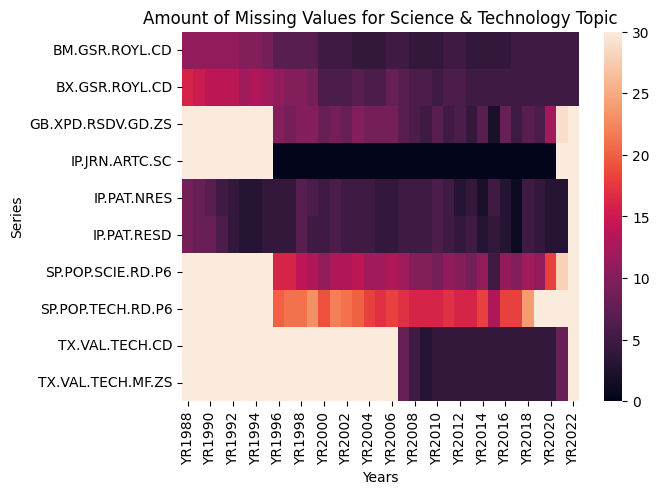
\includegraphics[width=0.7\textwidth]{Nan.png}
  \caption{Nan Analysis}
  \label{fig:nan}
\end{figure}

\clearpage
\section{Project Development} 
\subsection{Team Roles}
\begin{table}[H]
  \centering	
  \caption{Team Roles}
  \begin{tabular}{|p{5cm}|p{10cm}|}
    \hline
    \textbf{Role} & \textbf{Name} \\\hline
    Machine Learning & Gonzalo Ducca \\\hline
    Machine Learning & Carlos Madoery \\\hline
    Data Analytics & Valentino Caputa \\\hline
    Data Analytics & Juan P. Bertone \\\hline
    Data Engineer & Juan E. Flórez-Coronel \\\hline
  \end{tabular}
  \label{tab:teamroles}
\end{table}
\subsection{Gaant Chart}
\begin{figure}[htbp!]
  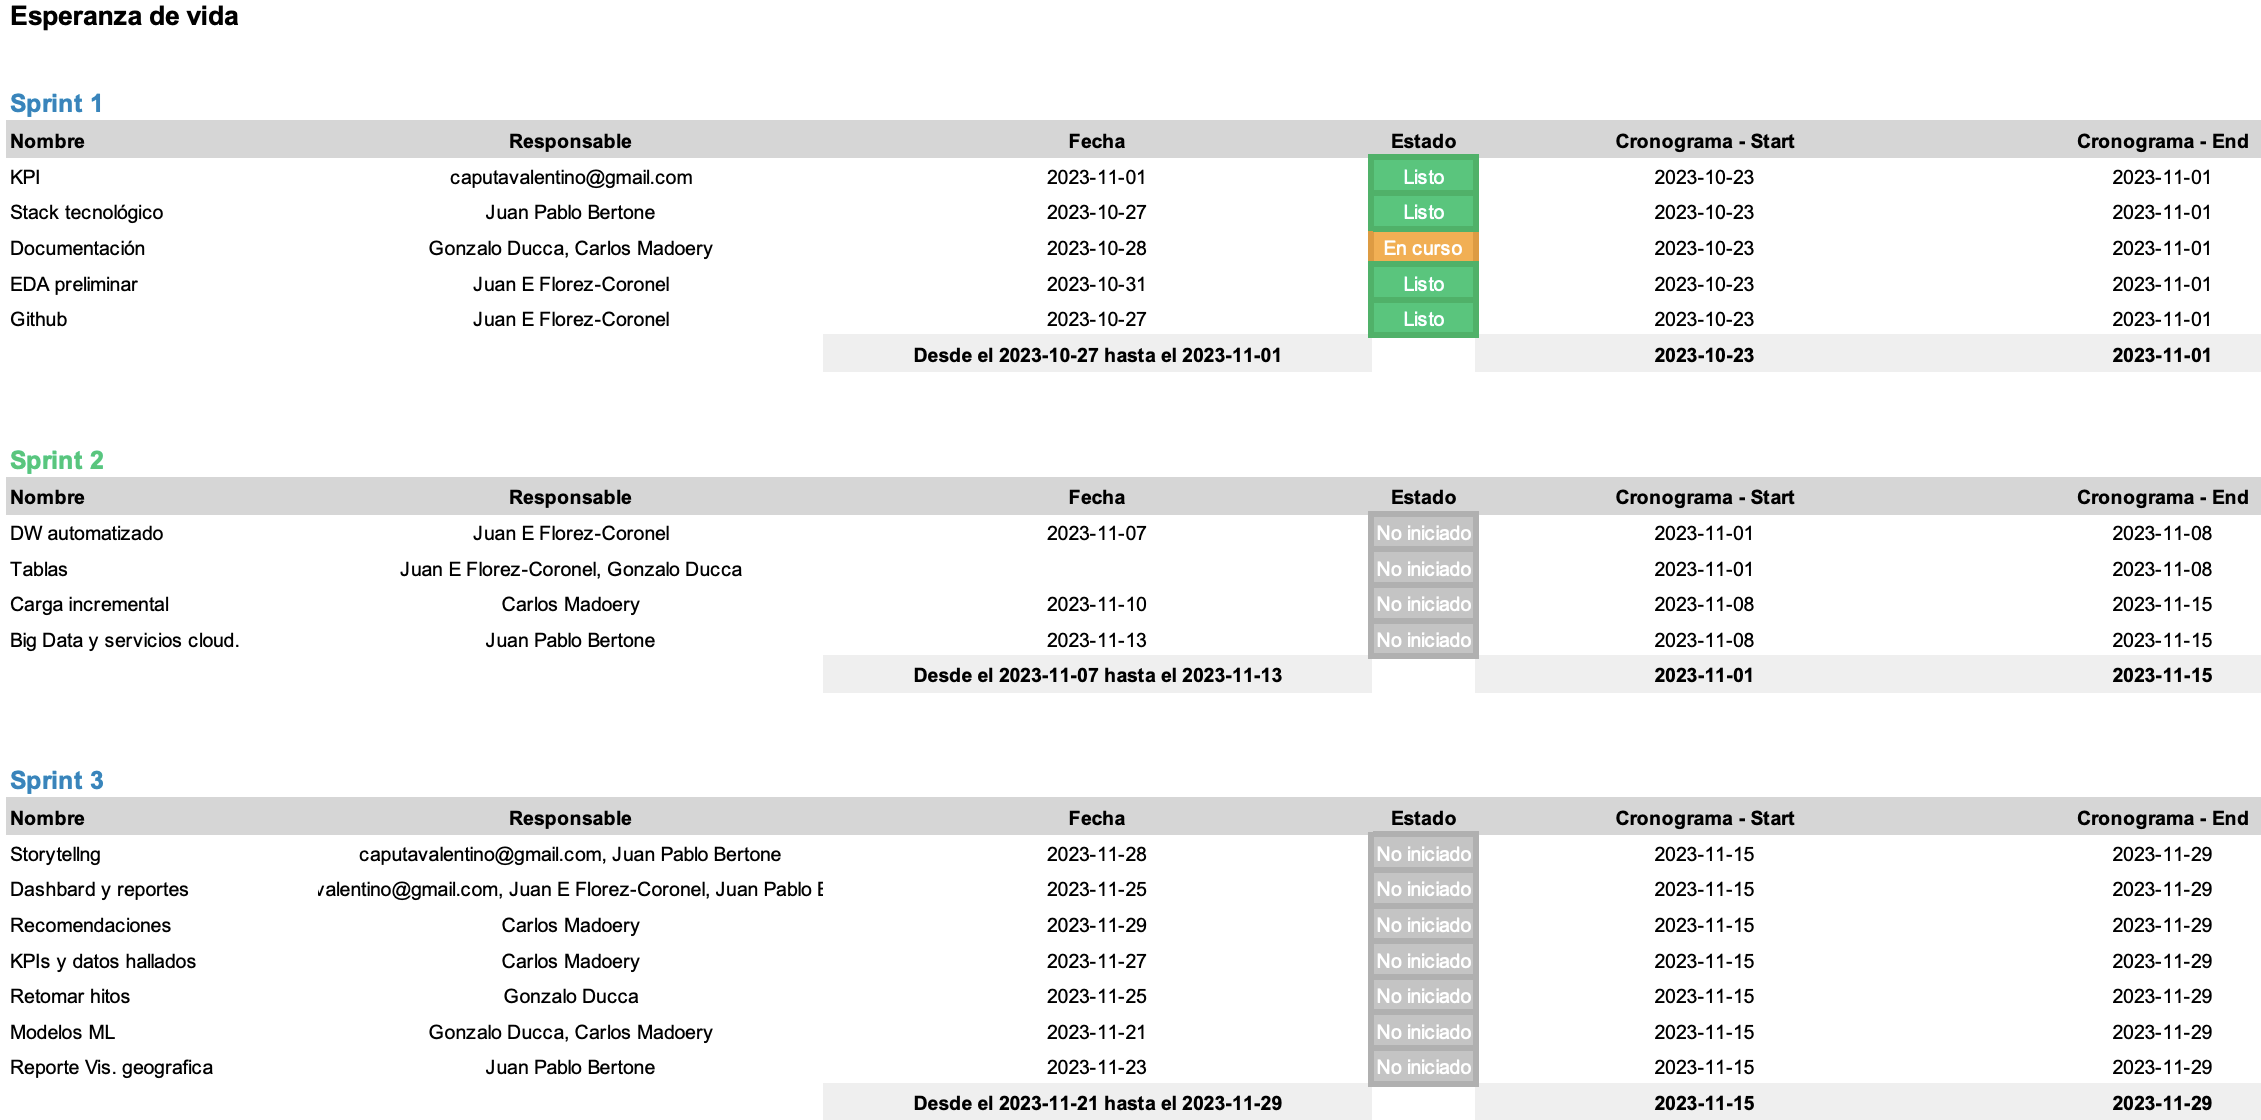
\includegraphics[width=\textwidth]{gaant.png}
  \caption{Project Gaant Chart}
  \label{fig:gaant}
\end{figure}

%%%%%%   Conclusions  %%%%%%  
\clearpage
\section*{Conclusions and Lessons Learned}
\addcontentsline{toc}{section}{Conclusions and Lessons Learned}%adds Conclusions and Lessons Learned section to the table of contents

bla

%----References-----%
%\clearpage
%Please refer to the OverLeaf Primer to see your options for how to keep track of references.
%\section*{References}
%\addcontentsline{toc}{section}{References}%adds reference section to the table of contents
%Use the OverLeaf Primer to understand the different ways to format the references. 
%\bibliographystyle{IEEEtran} %Formats the bibliography to meet the IEEE standards
%\bibliography{ref.bib} %This command calls a file named "your_references.bib". You will upload this file, and can rename as necessary. 
  

%\clearpage
%\appendix
% \renewcommand{\thesection}{\Alph{section}.}
%\setcounter{section}{0}

%\addcontentsline{toc}{section}{Appendices}
%--Product System Design Decomposition----% 
%\section{Product System Design Decomposition}
%Provide a complete design decomposition. If the different branches relate to different parts of the product design (i.e safety, electrical subsystem, mechanical subsystem, etc...), please label those to show at a high level an overview of your decomposition. 

%Uncomment and use the below commands to include your decomposition. The "angle=90" rotates the decomposition to a landscape view. 

%-----------Figure------------%
% \begin{figure}[ht!]
% \centering
% \includegraphics[width=1.1\textwidth, angle=90]{Design_Decomposition}
% \caption{System Design Map}
% \label{System Design Map}
% \end{figure}
%-------End of Figure---------%


%--Design Drawings/Schematics----% 
%\clearpage
%\section{Design Drawings/Schematics}
%Please provide necessary drawings and schematics here. These should include both the mechanical and electrical figures if applicable. 


%----Appendix Proof of Material Purchase---% 
%\clearpage
%\section{Proof of Material Purchases}
%Please provide a copy of your receipt(s) for the purchase of the items on your bill of materials. 

%----Appendix: Other---% 
%\clearpage
%\section{Other}

\end{document}
